\documentclass[border=10pt,varwidth=30cm]{standalone}
\usepackage{graphicx,capt-of}
\usepackage{rotating}
\usepackage{multirow}
\usepackage[cm]{sfmath}
\usepackage{xspace}

\renewcommand{\familydefault}{\sfdefault}

\newcounter{subfloat}
\renewcommand{\thesubfloat}{\Alph{subfloat}}
\newcommand{\image}[2]{%
    \stepcounter{subfloat}%
    \begin{tabular}[t]{@{}c@{}}
    \thesubfloat. #1 \\
    #2
    \end{tabular}%
}
\newcommand{\insertlabel}{%
    \small
    \stepcounter{subfloat}%
    \thesubfloat}
\newcommand{\trm}[1]{\ensuremath{\textrm{\sffamily #1}}}

\newcommand{\given}{\ensuremath{\,|\,}\xspace}
\newcommand{\pr}{\ensuremath{p}}

\newcommand{\ecoevolity}{ecoevolity\xspace}
\newcommand{\beast}{StarBEAST2\xspace}
\newcommand{\beastcore}{BEAST2\xspace}
\newcommand{\dendropy}{DendroPy\xspace}
\newcommand{\seqgen}{Seq-Gen\xspace}
\newcommand{\python}{Python\xspace}

\newcommand{\allsites}{all sites\xspace}
\newcommand{\snps}{SNPs\xspace}
\newcommand{\noerrors}{No errors}
\newcommand{\singletoneighty}{20\% singleton errors}
\newcommand{\singletonsixty}{40\% singleton errors}
\newcommand{\heteighty}{20\% het errors}
\newcommand{\hetsixty}{40\% het errors}


\newcommand{\data}{\ensuremath{D}\xspace}
\newcommand{\model}[1][]{\ensuremath{M_{#1}}\xspace}
\newcommand{\parameters}[1][]{\ensuremath{\Theta_{#1}}\xspace}
\newcommand{\parameter}[1][]{\ensuremath{\theta_{#1}}\xspace}
\newcommand{\diff}[1]{\ensuremath{\mathrm{d}#1}}

\newcommand{\distgamma}{\ensuremath{\textrm{Gamma}}\xspace}
\newcommand{\distexponential}{\ensuremath{\textrm{Exponential}}\xspace}
\newcommand{\dgamma}[2]{\ensuremath{\distgamma(\textrm{shape} = #1, \textrm{mean} = #2)}}
\newcommand{\dexponential}[1]{\ensuremath{\distexponential(\textrm{mean} = #1)}}
\newcommand{\gshape}{\ensuremath{k}\xspace}
\newcommand{\gscale}{\ensuremath{\theta}\xspace}

\newcommand{\nloci}[1][]{\ensuremath{m_{#1}\xspace}}

\newcommand{\observedallelecount}[1][]{\ensuremath{n_{#1}}\xspace}
\newcommand{\observedredallelecount}[1][]{\ensuremath{r_{#1}}\xspace}

\newcommand{\nodeallelecount}[2]{\ensuremath{n_{#1}^{#2}}}
\newcommand{\noderedallelecount}[2]{\ensuremath{r_{#1}^{#2}}}

\newcommand{\allelecount}[1][]{\ensuremath{\nodeallelecount{#1}{}}\xspace}
\newcommand{\redallelecount}[1][]{\ensuremath{\noderedallelecount{#1}{}}\xspace}

\newcommand{\leafallelecounts}[1][]{\ensuremath{\mathbf{n}_{#1}}\xspace}
\newcommand{\leafredallelecounts}[1][]{\ensuremath{\mathbf{r}_{#1}}\xspace}
\newcommand{\maxleafallelecounts}{\ensuremath{\textrm{max}(\mathbf{n})}\xspace}

\newcommand{\comparisondata}[1][]{\ensuremath{D_{#1}}\xspace}
\newcommand{\alldata}[1][]{\ensuremath{\mathbf{D}}\xspace}

\newcommand{\branchindex}{\ensuremath{x}\xspace}
\newcommand{\allelecountbottom}[1][\branchindex]{\nodeallelecount{#1}{B}}
\newcommand{\allelecounttop}[1][\branchindex]{\nodeallelecount{#1}{T}}
\newcommand{\redallelecountbottom}[1][\branchindex]{\noderedallelecount{#1}{B}}
\newcommand{\redallelecounttop}[1][\branchindex]{\noderedallelecount{#1}{T}}

\newcommand{\rgmurate}{\ensuremath{u}\xspace}
\newcommand{\grmurate}{\ensuremath{v}\xspace}
\newcommand{\murate}[1][]{\ensuremath{\mu_{#1}}\xspace}
\newcommand{\murates}[1][]{\ensuremath{\boldsymbol{\mu}_{#1}}\xspace}
\newcommand{\gfreq}[1][]{\ensuremath{\pi_{#1}}\xspace}
\newcommand{\gfreqs}[1][]{\ensuremath{\boldsymbol{\pi}_{#1}}\xspace}

\newcommand{\genetree}[1][]{\ensuremath{g_{#1}}\xspace}
\newcommand{\sptree}[1][]{\ensuremath{S_{#1}}\xspace}
\newcommand{\sptrees}[1][]{\ensuremath{\mathbf{S}_{#1}}\xspace}

\newcommand{\divtime}[1][]{\ensuremath{\tau_{#1}}\xspace}
\newcommand{\descendantpopindex}[1]{\ensuremath{D{#1}}}
\newcommand{\rootpopindex}[1][]{\ensuremath{R{#1}}\xspace}
\newcommand{\epopsize}[1][]{\ensuremath{N_{e}^{#1}}\xspace}
\newcommand{\rootpopsize}{\epopsize[\rootpopindex]\xspace}
\newcommand{\tippopsize}[1][]{\epopsize[\descendantpopindex{1}]\xspace}

% Fig reference with parentheses
\newcommand{\mainfigsp}{(\cref{fig:time1000,fig:time500,fig:time250,fig:roottheta1000,fig:roottheta500,fig:roottheta250,fig:theta1000,fig:theta500,fig:theta250})}
\newcommand{\timefigsp}{(\cref{fig:time1000,fig:time500,fig:time250})}
\newcommand{\thetafigsp}{(\cref{fig:theta1000,fig:theta500,fig:theta250})}
\newcommand{\rootfigsp}{(\cref{fig:roottheta1000,fig:roottheta500,fig:roottheta250})}

% Fig references without parentheses
\newcommand{\mainfigs}{\cref{fig:time1000,fig:time500,fig:time250,fig:roottheta1000,fig:roottheta500,fig:roottheta250,fig:theta1000,fig:theta500,fig:theta250}}
\newcommand{\timefigs}{\cref{fig:time1000,fig:time500,fig:time250}}
\newcommand{\thetafigs}{\cref{fig:theta1000,fig:theta500,fig:theta250}}
\newcommand{\rootfigs}{\cref{fig:roottheta1000,fig:roottheta500,fig:roottheta250}}

\begin{document}

\begin{figure}
    \centering
    \begin{tabular}{@{}cccccc@{}}
        \multicolumn{6}{c}{\LARGE 250bp loci} \\[2ex]
        & \multicolumn{1}{c}{\LARGE \beast}
        &
        & \multicolumn{2}{c}{\LARGE \ecoevolity}
        & \\
        \cline{2-2}\cline{4-5}
        & & & & & \\
        &
        &
        & \multicolumn{1}{c}{\Large \allsites}
        & \multicolumn{1}{c}{\Large \snps}
        & \\
        \multirow{5}{*}[-10em]{\begin{sideways}\Large Estimated descendant $N_e\mu$\end{sideways}}
        & 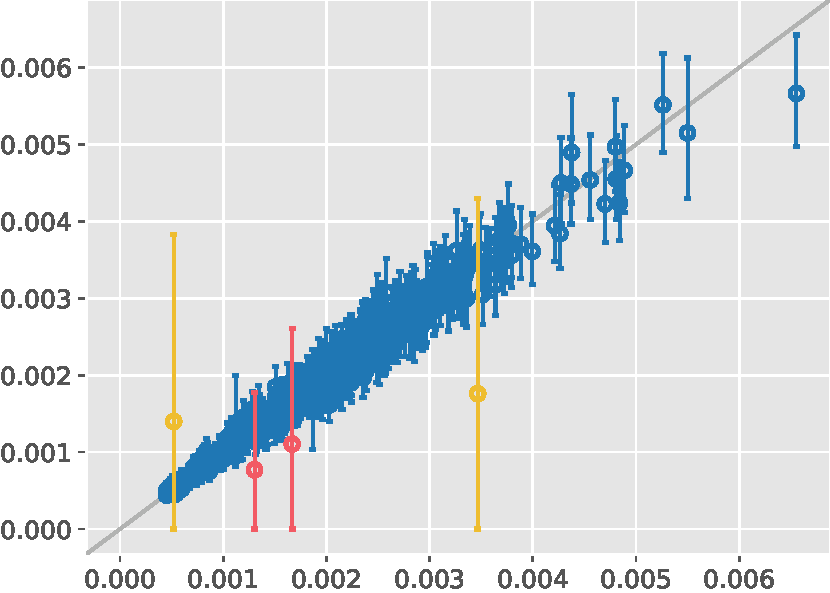
\includegraphics[width=0.18\textwidth]{{../out-sp2-gen4-loc400-len250/singleton-prob-1.0-starbeast-theta}.pdf}
        &
        & 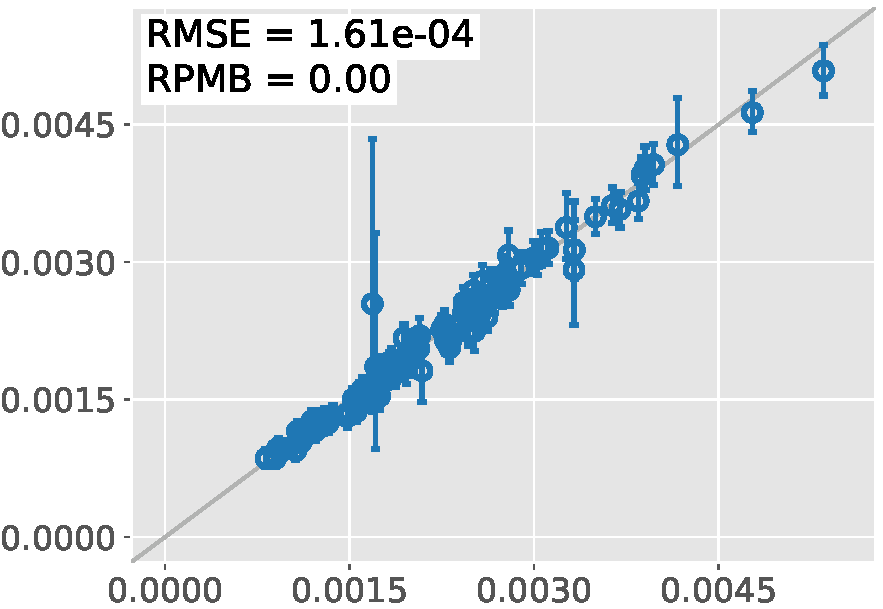
\includegraphics[width=0.18\textwidth]{{../out-sp2-gen4-loc400-len250/singleton-prob-1.0-ecoevolity-theta}.pdf}
        & 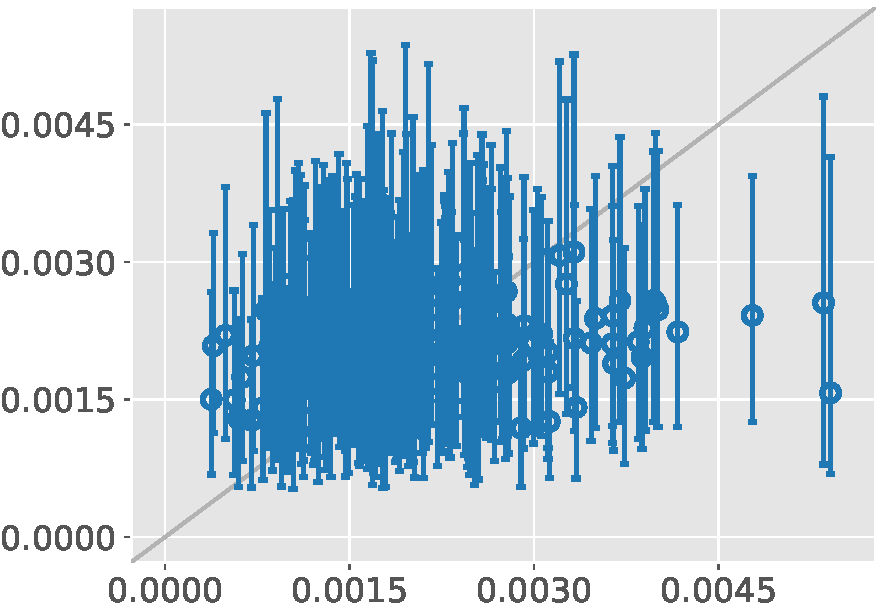
\includegraphics[width=0.18\textwidth]{{../out-sp2-gen4-loc400-len250/singleton-prob-1.0-snp-ecoevolity-theta}.pdf}
        & \multirow{1}{*}[7em]{\begin{sideways}\large \noerrors\end{sideways}} \\
        & 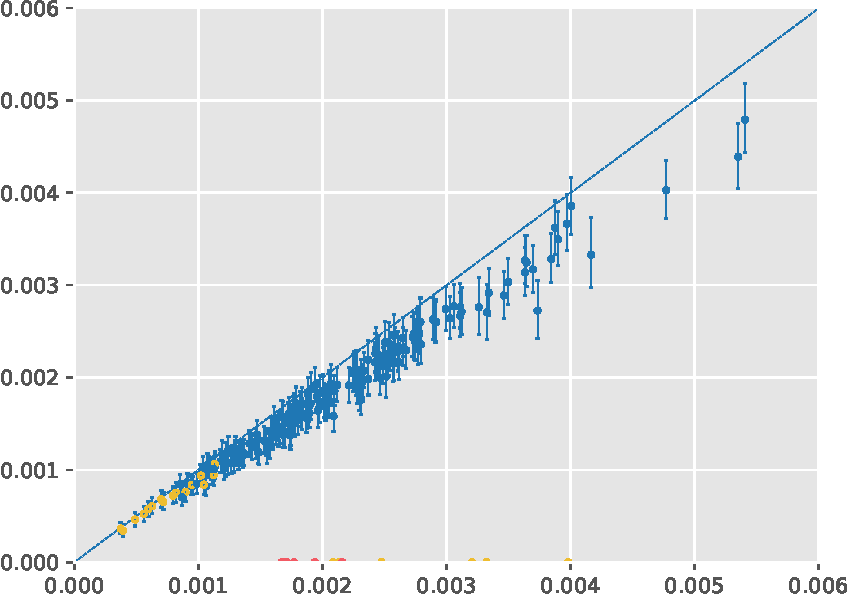
\includegraphics[width=0.18\textwidth]{{../out-sp2-gen4-loc400-len250/singleton-prob-0.8-starbeast-theta}.pdf}
        &
        & 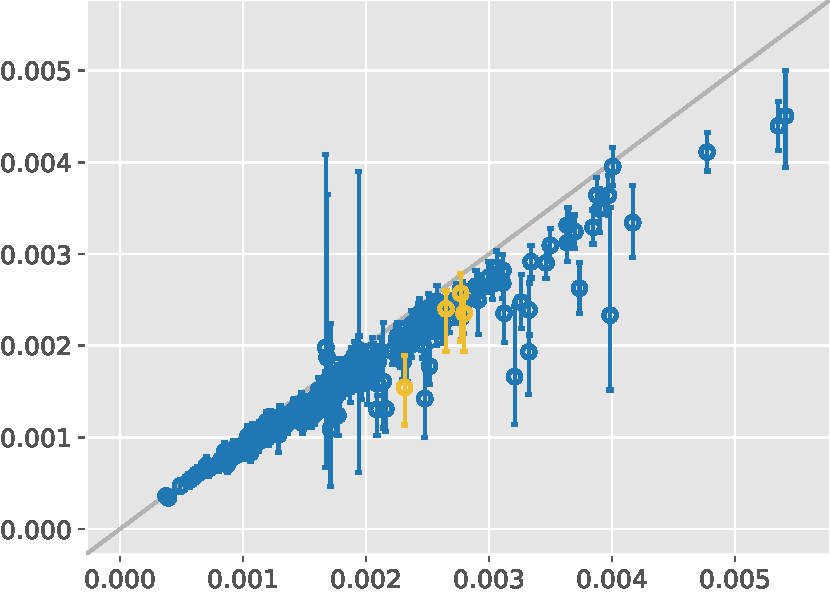
\includegraphics[width=0.18\textwidth]{{../out-sp2-gen4-loc400-len250/singleton-prob-0.8-ecoevolity-theta}.pdf}
        & 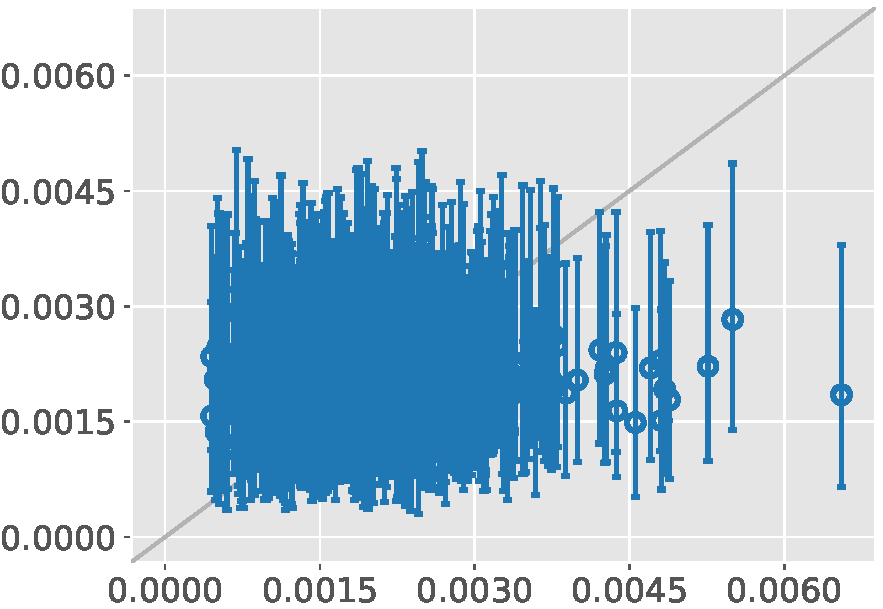
\includegraphics[width=0.18\textwidth]{{../out-sp2-gen4-loc400-len250/singleton-prob-0.8-snp-ecoevolity-theta}.pdf}
        & \multirow{1}{*}[10em]{\begin{sideways}\large \singletoneighty\end{sideways}} \\
        & 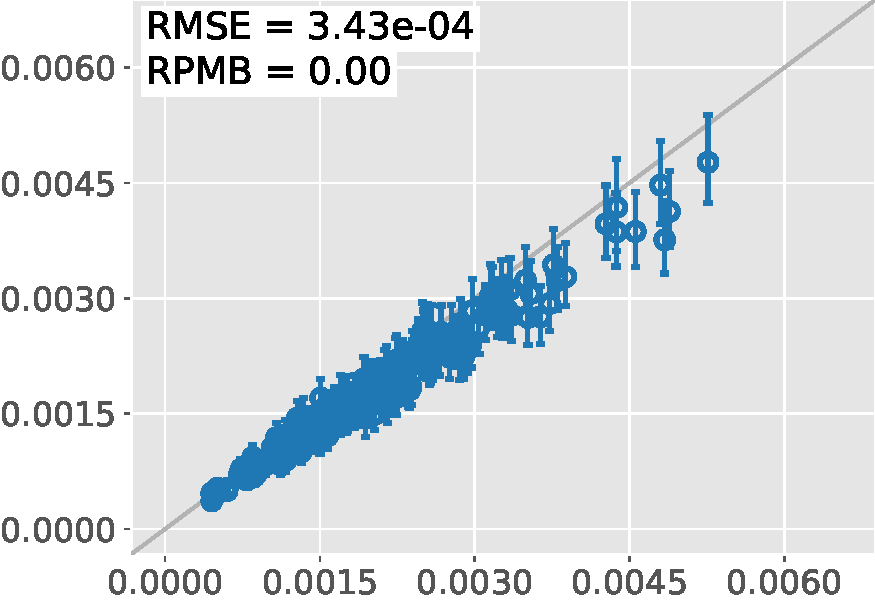
\includegraphics[width=0.18\textwidth]{{../out-sp2-gen4-loc400-len250/het-prob-0.8-starbeast-theta}.pdf}
        &
        & 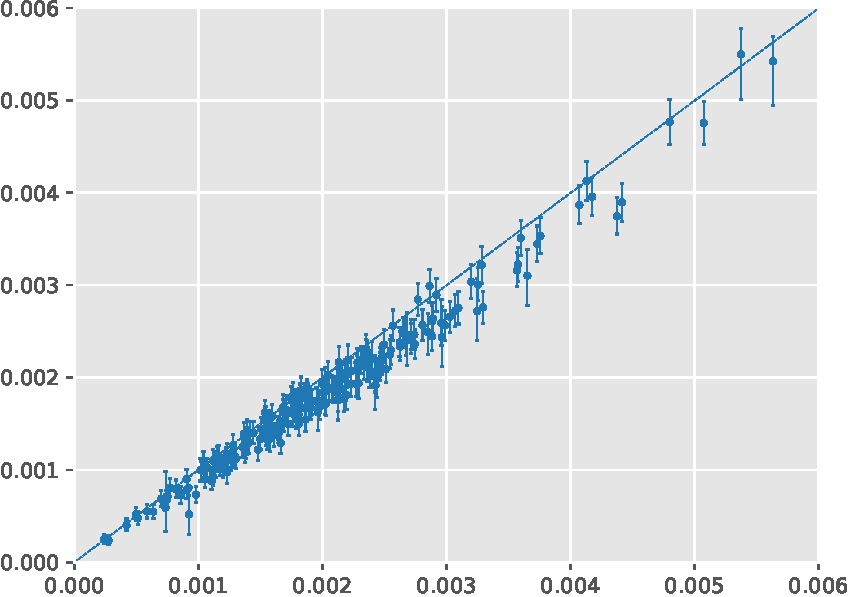
\includegraphics[width=0.18\textwidth]{{../out-sp2-gen4-loc400-len250/het-prob-0.8-ecoevolity-theta}.pdf}
        & 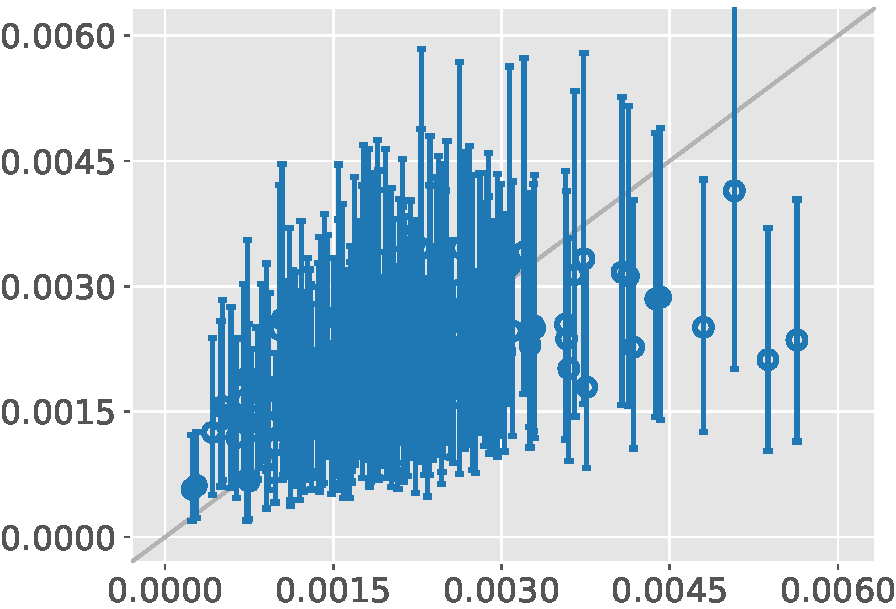
\includegraphics[width=0.18\textwidth]{{../out-sp2-gen4-loc400-len250/het-prob-0.8-snp-ecoevolity-theta}.pdf}
        & \multirow{1}{*}[8.5em]{\begin{sideways}\large \heteighty\end{sideways}} \\
        & 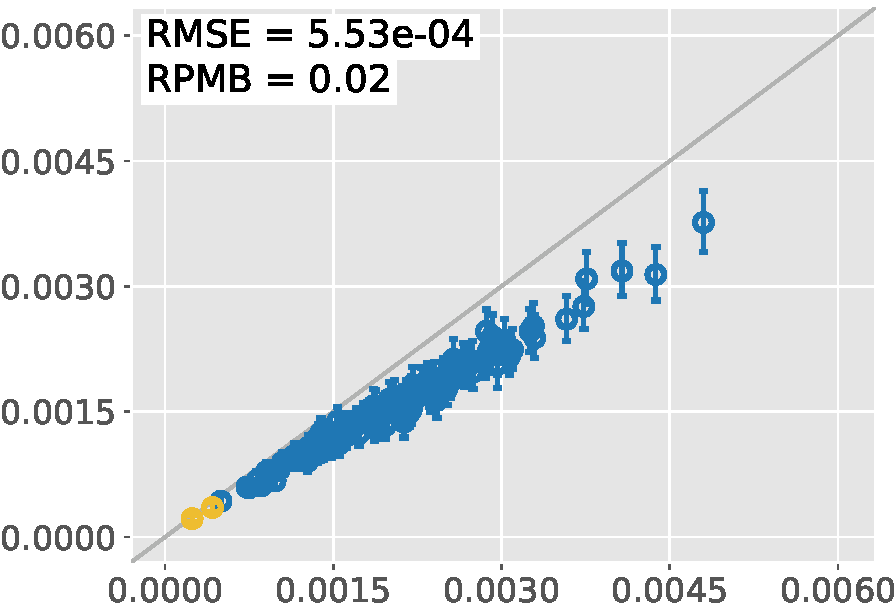
\includegraphics[width=0.18\textwidth]{{../out-sp2-gen4-loc400-len250/singleton-prob-0.6-starbeast-theta}.pdf}
        &
        & 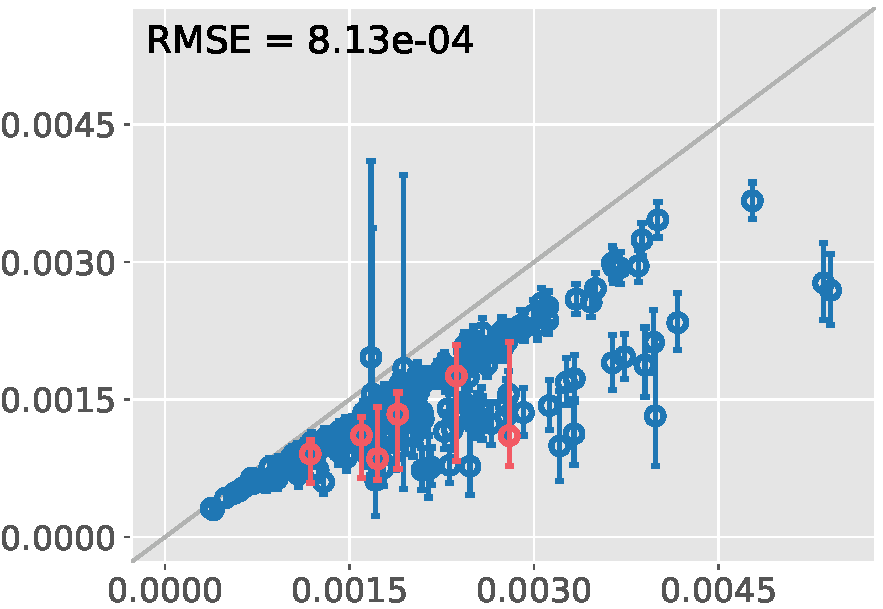
\includegraphics[width=0.18\textwidth]{{../out-sp2-gen4-loc400-len250/singleton-prob-0.6-ecoevolity-theta}.pdf}
        & 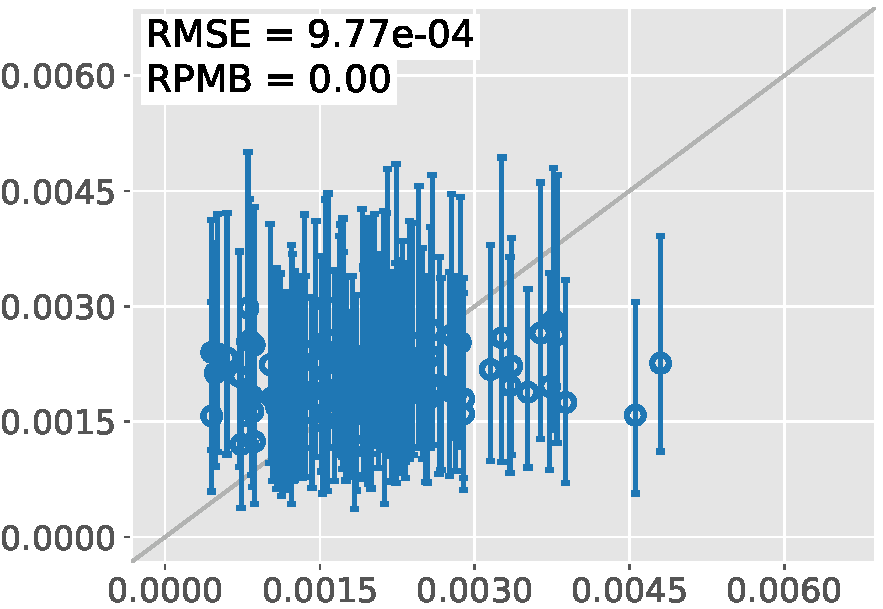
\includegraphics[width=0.18\textwidth]{{../out-sp2-gen4-loc400-len250/singleton-prob-0.6-snp-ecoevolity-theta}.pdf}
        & \multirow{1}{*}[10em]{\begin{sideways}\large \singletonsixty\end{sideways}} \\
        & 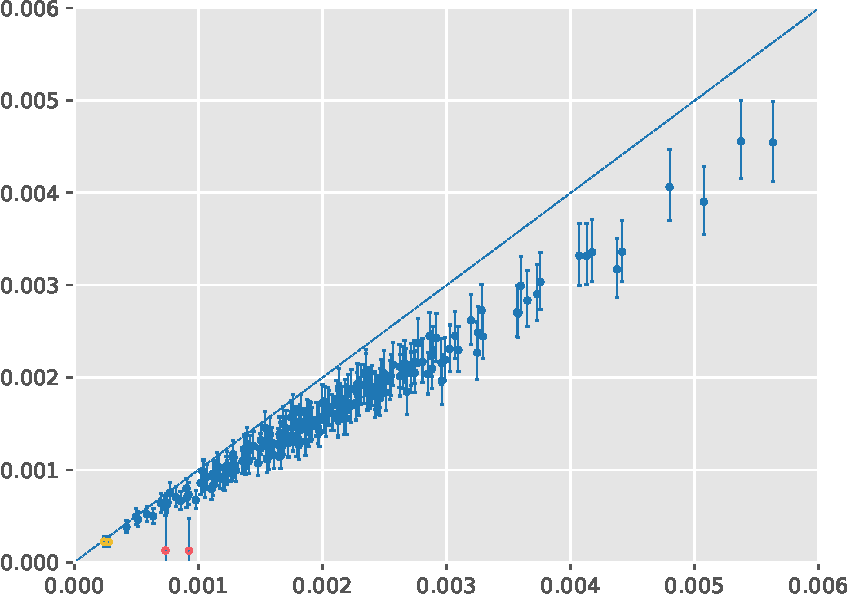
\includegraphics[width=0.18\textwidth]{{../out-sp2-gen4-loc400-len250/het-prob-0.6-starbeast-theta}.pdf}
        &
        & 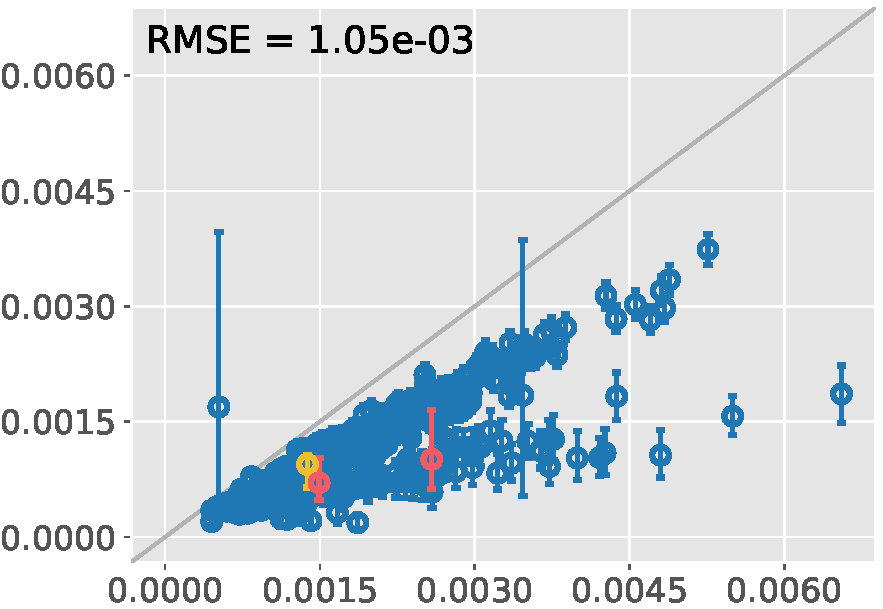
\includegraphics[width=0.18\textwidth]{{../out-sp2-gen4-loc400-len250/het-prob-0.6-ecoevolity-theta}.pdf}
        & 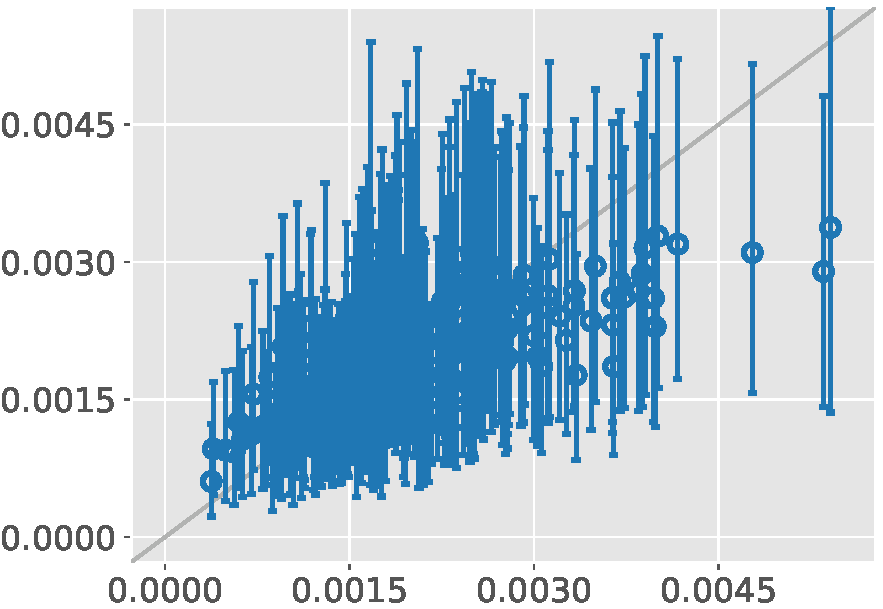
\includegraphics[width=0.18\textwidth]{{../out-sp2-gen4-loc400-len250/het-prob-0.6-snp-ecoevolity-theta}.pdf}
        & \multirow{1}{*}[8.5em]{\begin{sideways}\large \hetsixty\end{sideways}} \\
        & \multicolumn{4}{c}{\Large True descendant $N_e\mu$} & \\
    \end{tabular}
\end{figure}

\end{document}
